\documentclass[12pt,a4paper]{article}

\usepackage[a4paper,text={16.5cm,25.2cm},centering]{geometry}
\usepackage{lmodern}
\usepackage{amssymb,amsmath}
\usepackage{bm}
\usepackage{graphicx}
\usepackage{microtype}
\usepackage{hyperref}
\usepackage{mhchem}
\setlength{\parindent}{0pt}
\setlength{\parskip}{1.2ex}
\setcounter{secnumdepth}{0}% % Turns off numbering for sections
\hypersetup
       {
           colorlinks=TRUE,
           linkcolor=black,
           citecolor=blue,
           urlcolor=blue
       }

\usepackage{upquote}
\usepackage{listings}
\usepackage{xcolor}
\lstset{
    basicstyle=\ttfamily\footnotesize,
    upquote=true,
    breaklines=true,
    breakindent=0pt,
    keepspaces=true,
    showspaces=false,
    columns=fullflexible,
    showtabs=false,
    showstringspaces=false,
    escapeinside={(*@}{@*)},
    extendedchars=true,
}
\newcommand{\HLJLt}[1]{#1}
\newcommand{\HLJLw}[1]{#1}
\newcommand{\HLJLe}[1]{#1}
\newcommand{\HLJLeB}[1]{#1}
\newcommand{\HLJLo}[1]{#1}
\newcommand{\HLJLk}[1]{\textcolor[RGB]{148,91,176}{\textbf{#1}}}
\newcommand{\HLJLkc}[1]{\textcolor[RGB]{59,151,46}{\textit{#1}}}
\newcommand{\HLJLkd}[1]{\textcolor[RGB]{214,102,97}{\textit{#1}}}
\newcommand{\HLJLkn}[1]{\textcolor[RGB]{148,91,176}{\textbf{#1}}}
\newcommand{\HLJLkp}[1]{\textcolor[RGB]{148,91,176}{\textbf{#1}}}
\newcommand{\HLJLkr}[1]{\textcolor[RGB]{148,91,176}{\textbf{#1}}}
\newcommand{\HLJLkt}[1]{\textcolor[RGB]{148,91,176}{\textbf{#1}}}
\newcommand{\HLJLn}[1]{#1}
\newcommand{\HLJLna}[1]{#1}
\newcommand{\HLJLnb}[1]{#1}
\newcommand{\HLJLnbp}[1]{#1}
\newcommand{\HLJLnc}[1]{#1}
\newcommand{\HLJLncB}[1]{#1}
\newcommand{\HLJLnd}[1]{\textcolor[RGB]{214,102,97}{#1}}
\newcommand{\HLJLne}[1]{#1}
\newcommand{\HLJLneB}[1]{#1}
\newcommand{\HLJLnf}[1]{\textcolor[RGB]{66,102,213}{#1}}
\newcommand{\HLJLnfm}[1]{\textcolor[RGB]{66,102,213}{#1}}
\newcommand{\HLJLnp}[1]{#1}
\newcommand{\HLJLnl}[1]{#1}
\newcommand{\HLJLnn}[1]{#1}
\newcommand{\HLJLno}[1]{#1}
\newcommand{\HLJLnt}[1]{#1}
\newcommand{\HLJLnv}[1]{#1}
\newcommand{\HLJLnvc}[1]{#1}
\newcommand{\HLJLnvg}[1]{#1}
\newcommand{\HLJLnvi}[1]{#1}
\newcommand{\HLJLnvm}[1]{#1}
\newcommand{\HLJLl}[1]{#1}
\newcommand{\HLJLld}[1]{\textcolor[RGB]{148,91,176}{\textit{#1}}}
\newcommand{\HLJLs}[1]{\textcolor[RGB]{201,61,57}{#1}}
\newcommand{\HLJLsa}[1]{\textcolor[RGB]{201,61,57}{#1}}
\newcommand{\HLJLsb}[1]{\textcolor[RGB]{201,61,57}{#1}}
\newcommand{\HLJLsc}[1]{\textcolor[RGB]{201,61,57}{#1}}
\newcommand{\HLJLsd}[1]{\textcolor[RGB]{201,61,57}{#1}}
\newcommand{\HLJLsdB}[1]{\textcolor[RGB]{201,61,57}{#1}}
\newcommand{\HLJLsdC}[1]{\textcolor[RGB]{201,61,57}{#1}}
\newcommand{\HLJLse}[1]{\textcolor[RGB]{59,151,46}{#1}}
\newcommand{\HLJLsh}[1]{\textcolor[RGB]{201,61,57}{#1}}
\newcommand{\HLJLsi}[1]{#1}
\newcommand{\HLJLso}[1]{\textcolor[RGB]{201,61,57}{#1}}
\newcommand{\HLJLsr}[1]{\textcolor[RGB]{201,61,57}{#1}}
\newcommand{\HLJLss}[1]{\textcolor[RGB]{201,61,57}{#1}}
\newcommand{\HLJLssB}[1]{\textcolor[RGB]{201,61,57}{#1}}
\newcommand{\HLJLnB}[1]{\textcolor[RGB]{59,151,46}{#1}}
\newcommand{\HLJLnbB}[1]{\textcolor[RGB]{59,151,46}{#1}}
\newcommand{\HLJLnfB}[1]{\textcolor[RGB]{59,151,46}{#1}}
\newcommand{\HLJLnh}[1]{\textcolor[RGB]{59,151,46}{#1}}
\newcommand{\HLJLni}[1]{\textcolor[RGB]{59,151,46}{#1}}
\newcommand{\HLJLnil}[1]{\textcolor[RGB]{59,151,46}{#1}}
\newcommand{\HLJLnoB}[1]{\textcolor[RGB]{59,151,46}{#1}}
\newcommand{\HLJLoB}[1]{\textcolor[RGB]{102,102,102}{\textbf{#1}}}
\newcommand{\HLJLow}[1]{\textcolor[RGB]{102,102,102}{\textbf{#1}}}
\newcommand{\HLJLp}[1]{#1}
\newcommand{\HLJLc}[1]{\textcolor[RGB]{153,153,119}{\textit{#1}}}
\newcommand{\HLJLch}[1]{\textcolor[RGB]{153,153,119}{\textit{#1}}}
\newcommand{\HLJLcm}[1]{\textcolor[RGB]{153,153,119}{\textit{#1}}}
\newcommand{\HLJLcp}[1]{\textcolor[RGB]{153,153,119}{\textit{#1}}}
\newcommand{\HLJLcpB}[1]{\textcolor[RGB]{153,153,119}{\textit{#1}}}
\newcommand{\HLJLcs}[1]{\textcolor[RGB]{153,153,119}{\textit{#1}}}
\newcommand{\HLJLcsB}[1]{\textcolor[RGB]{153,153,119}{\textit{#1}}}
\newcommand{\HLJLg}[1]{#1}
\newcommand{\HLJLgd}[1]{#1}
\newcommand{\HLJLge}[1]{#1}
\newcommand{\HLJLgeB}[1]{#1}
\newcommand{\HLJLgh}[1]{#1}
\newcommand{\HLJLgi}[1]{#1}
\newcommand{\HLJLgo}[1]{#1}
\newcommand{\HLJLgp}[1]{#1}
\newcommand{\HLJLgs}[1]{#1}
\newcommand{\HLJLgsB}[1]{#1}
\newcommand{\HLJLgt}[1]{#1}


\begin{document}

\section{Ordinary differential equation model with inference}
Simon Frost (@sdwfrost), 2020-04-27

\subsection{Introduction}
The classical ODE version of the SIR model is:

\begin{itemize}
\item Deterministic


\item Continuous in time


\item Continuous in state

\end{itemize}
In this notebook, we try to infer the parameter values from a simulated dataset.

\subsection{Libraries}

\begin{lstlisting}
(*@\HLJLk{using}@*) (*@\HLJLn{DifferentialEquations}@*)
(*@\HLJLk{using}@*) (*@\HLJLn{SimpleDiffEq}@*)
(*@\HLJLk{using}@*) (*@\HLJLn{DiffEqCallbacks}@*)
(*@\HLJLk{using}@*) (*@\HLJLn{Random}@*)
(*@\HLJLk{using}@*) (*@\HLJLn{Distributions}@*)
(*@\HLJLk{using}@*) (*@\HLJLn{DiffEqParamEstim}@*)
(*@\HLJLk{using}@*) (*@\HLJLn{DataFrames}@*)
(*@\HLJLk{using}@*) (*@\HLJLn{StatsPlots}@*)
(*@\HLJLk{using}@*) (*@\HLJLn{BenchmarkTools}@*)
\end{lstlisting}


\subsection{Transitions}
The following function provides the derivatives of the model, which it changes in-place. State variables and parameters are unpacked from \texttt{u} and \texttt{p}; this incurs a slight performance hit, but makes the equations much easier to read.

A variable is included for the number of infections, $Y$.


\begin{lstlisting}
(*@\HLJLk{function}@*) (*@\HLJLnf{sir{\_}ode!}@*)(*@\HLJLp{(}@*)(*@\HLJLn{du}@*)(*@\HLJLp{,}@*)(*@\HLJLn{u}@*)(*@\HLJLp{,}@*)(*@\HLJLn{p}@*)(*@\HLJLp{,}@*)(*@\HLJLn{t}@*)(*@\HLJLp{)}@*)
    (*@\HLJLp{(}@*)(*@\HLJLn{S}@*)(*@\HLJLp{,}@*)(*@\HLJLn{I}@*)(*@\HLJLp{,}@*)(*@\HLJLn{R}@*)(*@\HLJLp{,}@*)(*@\HLJLn{Y}@*)(*@\HLJLp{)}@*) (*@\HLJLoB{=}@*) (*@\HLJLn{u}@*)
    (*@\HLJLp{(}@*)(*@\HLJLn{\ensuremath{\beta}}@*)(*@\HLJLp{,}@*)(*@\HLJLn{c}@*)(*@\HLJLp{,}@*)(*@\HLJLn{\ensuremath{\gamma}}@*)(*@\HLJLp{)}@*) (*@\HLJLoB{=}@*) (*@\HLJLn{p}@*)
    (*@\HLJLn{N}@*) (*@\HLJLoB{=}@*) (*@\HLJLn{S}@*)(*@\HLJLoB{+}@*)(*@\HLJLn{I}@*)(*@\HLJLoB{+}@*)(*@\HLJLn{R}@*)
    (*@\HLJLn{infection}@*) (*@\HLJLoB{=}@*) (*@\HLJLn{\ensuremath{\beta}}@*)(*@\HLJLoB{*}@*)(*@\HLJLn{c}@*)(*@\HLJLoB{*}@*)(*@\HLJLn{I}@*)(*@\HLJLoB{/}@*)(*@\HLJLn{N}@*)(*@\HLJLoB{*}@*)(*@\HLJLn{S}@*)
    (*@\HLJLn{recovery}@*) (*@\HLJLoB{=}@*) (*@\HLJLn{\ensuremath{\gamma}}@*)(*@\HLJLoB{*}@*)(*@\HLJLn{I}@*)
    (*@\HLJLnd{@inbounds}@*) (*@\HLJLk{begin}@*)
        (*@\HLJLn{du}@*)(*@\HLJLp{[}@*)(*@\HLJLni{1}@*)(*@\HLJLp{]}@*) (*@\HLJLoB{=}@*) (*@\HLJLoB{-}@*)(*@\HLJLn{infection}@*)
        (*@\HLJLn{du}@*)(*@\HLJLp{[}@*)(*@\HLJLni{2}@*)(*@\HLJLp{]}@*) (*@\HLJLoB{=}@*) (*@\HLJLn{infection}@*) (*@\HLJLoB{-}@*) (*@\HLJLn{recovery}@*)
        (*@\HLJLn{du}@*)(*@\HLJLp{[}@*)(*@\HLJLni{3}@*)(*@\HLJLp{]}@*) (*@\HLJLoB{=}@*) (*@\HLJLn{recovery}@*)
        (*@\HLJLn{du}@*)(*@\HLJLp{[}@*)(*@\HLJLni{4}@*)(*@\HLJLp{]}@*) (*@\HLJLoB{=}@*) (*@\HLJLn{infection}@*)
    (*@\HLJLk{end}@*)
    (*@\HLJLn{nothing}@*)
(*@\HLJLk{end}@*)(*@\HLJLp{;}@*)
\end{lstlisting}

\begin{lstlisting}
sir(*@{{\_}}@*)ode! (generic function with 1 method)
\end{lstlisting}


\subsection{Time domain}
We set the timespan for simulations, \texttt{tspan}, initial conditions, \texttt{u0}, and parameter values, \texttt{p} (which are unpacked above as \texttt{[\ensuremath{\beta},\ensuremath{\gamma}]}).


\begin{lstlisting}
(*@\HLJLn{\ensuremath{\delta}t}@*) (*@\HLJLoB{=}@*) (*@\HLJLnfB{0.1}@*)
(*@\HLJLn{tmax}@*) (*@\HLJLoB{=}@*) (*@\HLJLnfB{40.0}@*)
(*@\HLJLn{tspan}@*) (*@\HLJLoB{=}@*) (*@\HLJLp{(}@*)(*@\HLJLnfB{0.0}@*)(*@\HLJLp{,}@*)(*@\HLJLn{tmax}@*)(*@\HLJLp{)}@*)
(*@\HLJLn{t}@*) (*@\HLJLoB{=}@*) (*@\HLJLnfB{0.0}@*)(*@\HLJLoB{:}@*)(*@\HLJLn{\ensuremath{\delta}t}@*)(*@\HLJLoB{:}@*)(*@\HLJLn{tmax}@*)
(*@\HLJLn{obstimes}@*) (*@\HLJLoB{=}@*) (*@\HLJLni{0}@*)(*@\HLJLoB{:}@*)(*@\HLJLnfB{1.0}@*)(*@\HLJLoB{:}@*)(*@\HLJLn{tmax}@*)(*@\HLJLp{;}@*)
\end{lstlisting}

\begin{lstlisting}
0.0:1.0:40.0
\end{lstlisting}


\subsection{Initial conditions}

\begin{lstlisting}
(*@\HLJLn{u0}@*) (*@\HLJLoB{=}@*) (*@\HLJLp{[}@*)(*@\HLJLnfB{990.0}@*)(*@\HLJLp{,}@*)(*@\HLJLnfB{10.0}@*)(*@\HLJLp{,}@*)(*@\HLJLnfB{0.0}@*)(*@\HLJLp{,}@*)(*@\HLJLnfB{0.0}@*)(*@\HLJLp{];}@*) (*@\HLJLcs{{\#}}@*) (*@\HLJLcs{S,I.R,Y}@*)
\end{lstlisting}

\begin{lstlisting}
4-element Array(*@{{\{}}@*)Float64,1(*@{{\}}}@*):
 990.0
  10.0
   0.0
   0.0
\end{lstlisting}


\subsection{Parameter values}

\begin{lstlisting}
(*@\HLJLn{p}@*) (*@\HLJLoB{=}@*) (*@\HLJLp{[}@*)(*@\HLJLnfB{0.05}@*)(*@\HLJLp{,}@*)(*@\HLJLnfB{10.0}@*)(*@\HLJLp{,}@*)(*@\HLJLnfB{0.25}@*)(*@\HLJLp{];}@*) (*@\HLJLcs{{\#}}@*) (*@\HLJLcs{\ensuremath{\beta},c,\ensuremath{\gamma}}@*)
\end{lstlisting}

\begin{lstlisting}
3-element Array(*@{{\{}}@*)Float64,1(*@{{\}}}@*):
  0.05
 10.0
  0.25
\end{lstlisting}


\subsection{Accumulator interface}
In order to fit counts of new infections every time unit, we add a callback that sets $Y$ to zero at the observation times. This will result in two observations (one with non-zero \texttt{Y}, one with \texttt{Y}=0) at each observation time. However, the standard saving behaviour is turned off, so we don't need to have a special saving callback.


\begin{lstlisting}
(*@\HLJLnf{affect!}@*)(*@\HLJLp{(}@*)(*@\HLJLn{integrator}@*)(*@\HLJLp{)}@*) (*@\HLJLoB{=}@*) (*@\HLJLn{integrator}@*)(*@\HLJLoB{.}@*)(*@\HLJLn{u}@*)(*@\HLJLp{[}@*)(*@\HLJLni{4}@*)(*@\HLJLp{]}@*) (*@\HLJLoB{=}@*) (*@\HLJLnfB{0.0}@*)
(*@\HLJLn{cb{\_}zero}@*) (*@\HLJLoB{=}@*) (*@\HLJLnf{PresetTimeCallback}@*)(*@\HLJLp{(}@*)(*@\HLJLn{obstimes}@*)(*@\HLJLp{,}@*)(*@\HLJLn{affect!}@*)(*@\HLJLp{)}@*)
\end{lstlisting}

\begin{lstlisting}
DiscreteCallback(*@{{\{}}@*)DiffEqCallbacks.var(*@{"{}}@*)(*@{{\#}}@*)53(*@{{\#}}@*)56(*@{"{}}@*)(*@{{\{}}@*)StepRangeLen(*@{{\{}}@*)Float64,Base.Twic
ePrecision(*@{{\{}}@*)Float64(*@{{\}}}@*),Base.TwicePrecision(*@{{\{}}@*)Float64(*@{{\}}}@*)(*@{{\}}}@*)(*@{{\}}}@*),DiffEqCallbacks.var(*@{"{}}@*)(*@{{\#}}@*)54(*@{{\#}}@*)
57(*@{"{}}@*)(*@{{\{}}@*)typeof(Main.(*@{{\#}}@*)(*@{{\#}}@*)WeaveSandBox(*@{{\#}}@*)993.affect!)(*@{{\}}}@*),DiffEqCallbacks.var(*@{"{}}@*)(*@{{\#}}@*)55(*@{{\#}}@*)58(*@{"{}}@*)(*@{{\{}}@*)ty
peof(DiffEqBase.INITIALIZE(*@{{\_}}@*)DEFAULT),Bool,StepRangeLen(*@{{\{}}@*)Float64,Base.TwicePre
cision(*@{{\{}}@*)Float64(*@{{\}}}@*),Base.TwicePrecision(*@{{\{}}@*)Float64(*@{{\}}}@*)(*@{{\}}}@*),typeof(Main.(*@{{\#}}@*)(*@{{\#}}@*)WeaveSandBox(*@{{\#}}@*)99
3.affect!)(*@{{\}}}@*)(*@{{\}}}@*)(DiffEqCallbacks.var(*@{"{}}@*)(*@{{\#}}@*)53(*@{{\#}}@*)56(*@{"{}}@*)(*@{{\{}}@*)StepRangeLen(*@{{\{}}@*)Float64,Base.TwicePre
cision(*@{{\{}}@*)Float64(*@{{\}}}@*),Base.TwicePrecision(*@{{\{}}@*)Float64(*@{{\}}}@*)(*@{{\}}}@*)(*@{{\}}}@*)(0.0:1.0:40.0), DiffEqCallbac
ks.var(*@{"{}}@*)(*@{{\#}}@*)54(*@{{\#}}@*)57(*@{"{}}@*)(*@{{\{}}@*)typeof(Main.(*@{{\#}}@*)(*@{{\#}}@*)WeaveSandBox(*@{{\#}}@*)993.affect!)(*@{{\}}}@*)(Main.(*@{{\#}}@*)(*@{{\#}}@*)WeaveSandBox
(*@{{\#}}@*)993.affect!), DiffEqCallbacks.var(*@{"{}}@*)(*@{{\#}}@*)55(*@{{\#}}@*)58(*@{"{}}@*)(*@{{\{}}@*)typeof(DiffEqBase.INITIALIZE(*@{{\_}}@*)DEF
AULT),Bool,StepRangeLen(*@{{\{}}@*)Float64,Base.TwicePrecision(*@{{\{}}@*)Float64(*@{{\}}}@*),Base.TwicePrec
ision(*@{{\{}}@*)Float64(*@{{\}}}@*)(*@{{\}}}@*),typeof(Main.(*@{{\#}}@*)(*@{{\#}}@*)WeaveSandBox(*@{{\#}}@*)993.affect!)(*@{{\}}}@*)(DiffEqBase.INITIAL
IZE(*@{{\_}}@*)DEFAULT, true, 0.0:1.0:40.0, Main.(*@{{\#}}@*)(*@{{\#}}@*)WeaveSandBox(*@{{\#}}@*)993.affect!), Bool[1, 
1])
\end{lstlisting}


\subsection{Running the model}

\begin{lstlisting}
(*@\HLJLn{prob{\_}ode}@*) (*@\HLJLoB{=}@*) (*@\HLJLnf{ODEProblem}@*)(*@\HLJLp{(}@*)(*@\HLJLn{sir{\_}ode!}@*)(*@\HLJLp{,}@*)(*@\HLJLn{u0}@*)(*@\HLJLp{,}@*)(*@\HLJLn{tspan}@*)(*@\HLJLp{,}@*)(*@\HLJLn{p}@*)(*@\HLJLp{)}@*)
\end{lstlisting}

\begin{lstlisting}
ODEProblem with uType Array(*@{{\{}}@*)Float64,1(*@{{\}}}@*) and tType Float64. In-place: true
timespan: (0.0, 40.0)
u0: [990.0, 10.0, 0.0, 0.0]
\end{lstlisting}


The callback that resets \texttt{Y} is added to the system. Note that this requires \texttt{DiffEqCallbacks}. If multiple callbacks are required, then a \texttt{CallbackSet} can be passed instead.


\begin{lstlisting}
(*@\HLJLn{sol{\_}ode}@*) (*@\HLJLoB{=}@*) (*@\HLJLnf{solve}@*)(*@\HLJLp{(}@*)(*@\HLJLn{prob{\_}ode}@*)(*@\HLJLp{,}@*)(*@\HLJLn{callback}@*)(*@\HLJLoB{=}@*)(*@\HLJLn{cb{\_}zero}@*)(*@\HLJLp{);}@*)
\end{lstlisting}

\begin{lstlisting}
retcode: Success
Interpolation: Automatic order switching interpolation
t: 91-element Array(*@{{\{}}@*)Float64,1(*@{{\}}}@*):
  0.0
  0.00025500744028082863
  0.0028050818430891146
  0.028305825871171975
  0.26073498995506483
  0.879745906272606
  1.0
  1.0
  1.6085137638559268
  2.0
  (*@\ensuremath{\vdots}@*)
 36.0
 37.0
 37.0
 38.0
 38.0
 39.0
 39.0
 40.0
 40.0
u: 91-element Array(*@{{\{}}@*)Array(*@{{\{}}@*)Float64,1(*@{{\}}}@*),1(*@{{\}}}@*):
 [990.0, 10.0, 0.0, 0.0]
 [989.9987376745428, 10.000624786941064, 0.0006375385161680651, 0.001262325
4572314987]
 [989.9861101700155, 10.006874715124146, 0.007015114860333896, 0.0138898299
84480533]
 [989.859409227541, 10.069580289573166, 0.07101048288583331, 0.140590772458
99926]
 [988.6681819993325, 10.658729802298323, 0.6730881983691819, 1.331818000667
5044]
 [985.153961706524, 12.392534359288648, 2.453503934187351, 4.84603829347599
8]
 [984.4093729528591, 12.759075463490184, 2.8315515836506275, 5.590627047140
812]
 [984.4093729528591, 12.759075463490184, 2.8315515836506275, 0.0]
 [980.3013361862652, 14.77619740366821, 4.922466410066549, 4.10803676659394
8]
 [977.3332016509414, 16.228146587606428, 6.438651761452043, 7.0761713019176
61]
 (*@\ensuremath{\vdots}@*)
 [218.20787301998945, 25.66373329519949, 756.1283936848109, 0.0]
 [215.61229424401364, 22.27616524756678, 762.1115405084195, 2.5955787759757
976]
 [215.61229424401364, 22.27616524756678, 762.1115405084195, 0.0]
 [213.3857061722601, 19.312500522282374, 767.3017933054574, 2.2265880717535
4]
 [213.3857061722601, 19.312500522282374, 767.3017933054574, 0.0]
 [211.4749483263679, 16.725852658521724, 771.7991990151103, 1.9107578458921
968]
 [211.4749483263679, 16.725852658521724, 771.7991990151103, 0.0]
 [209.834667019888, 14.472822400047164, 775.6925105800648, 1.64028130647990
62]
 [209.834667019888, 14.472822400047164, 775.6925105800648, 0.0]
\end{lstlisting}


\subsection{Post-processing}
We can convert the output to a dataframe for convenience.


\begin{lstlisting}
(*@\HLJLn{df{\_}ode}@*) (*@\HLJLoB{=}@*) (*@\HLJLnf{DataFrame}@*)(*@\HLJLp{(}@*)(*@\HLJLnf{sol{\_}ode}@*)(*@\HLJLp{(}@*)(*@\HLJLn{obstimes}@*)(*@\HLJLp{)}@*)(*@\HLJLoB{{\textquotesingle}}@*)(*@\HLJLp{)}@*)
(*@\HLJLn{df{\_}ode}@*)(*@\HLJLp{[}@*)(*@\HLJLoB{!}@*)(*@\HLJLp{,}@*)(*@\HLJLoB{:}@*)(*@\HLJLn{t}@*)(*@\HLJLp{]}@*) (*@\HLJLoB{=}@*) (*@\HLJLn{obstimes}@*)(*@\HLJLp{;}@*)
\end{lstlisting}

\begin{lstlisting}
0.0:1.0:40.0
\end{lstlisting}


\subsection{Plotting}
We can now plot the results.


\begin{lstlisting}
(*@\HLJLnd{@df}@*) (*@\HLJLn{df{\_}ode}@*) (*@\HLJLnf{plot}@*)(*@\HLJLp{(}@*)(*@\HLJLsc{:t}@*)(*@\HLJLp{,}@*)
    (*@\HLJLp{[}@*)(*@\HLJLsc{:x1}@*) (*@\HLJLsc{:x2}@*) (*@\HLJLsc{:x3}@*) (*@\HLJLsc{:x4}@*)(*@\HLJLp{],}@*)
    (*@\HLJLn{label}@*)(*@\HLJLoB{=}@*)(*@\HLJLp{[}@*)(*@\HLJLs{"{}S"{}}@*) (*@\HLJLs{"{}I"{}}@*) (*@\HLJLs{"{}R"{}}@*) (*@\HLJLs{"{}Y"{}}@*)(*@\HLJLp{],}@*)
    (*@\HLJLn{xlabel}@*)(*@\HLJLoB{=}@*)(*@\HLJLs{"{}Time"{}}@*)(*@\HLJLp{,}@*)
    (*@\HLJLn{ylabel}@*)(*@\HLJLoB{=}@*)(*@\HLJLs{"{}Number"{}}@*)(*@\HLJLp{)}@*)
\end{lstlisting}

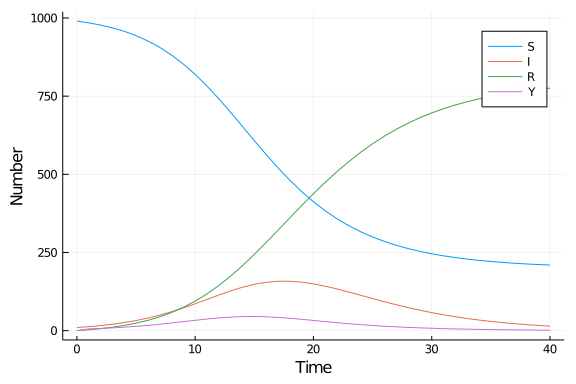
\includegraphics[width=\linewidth]{/home/simon/Projects/sir-julia/pdf/ode/jl_X4tZiv/ode_inference_10_1.pdf}

\subsection{Generating data}
Although the ODE system is deterministic, we can add measurement error to the counts of new cases. Here, a Poisson distribution is used, although a negative binomial could also be used (which would introduce an additional parameter for the variance).


\begin{lstlisting}
(*@\HLJLn{Random}@*)(*@\HLJLoB{.}@*)(*@\HLJLnf{seed!}@*)(*@\HLJLp{(}@*)(*@\HLJLni{1234}@*)(*@\HLJLp{);}@*)
\end{lstlisting}

\begin{lstlisting}
MersenneTwister(UInt32[0x000004d2], Random.DSFMT.DSFMT(*@{{\_}}@*)state(Int32[-1393240
018, 1073611148, 45497681, 1072875908, 436273599, 1073674613, -2043716458, 
1073445557, -254908435, 1072827086  (*@\ensuremath{\dots}@*)  -599655111, 1073144102, 367655457, 1
072985259, -1278750689, 1018350124, -597141475, 249849711, 382, 0]), [0.0, 
0.0, 0.0, 0.0, 0.0, 0.0, 0.0, 0.0, 0.0, 0.0  (*@\ensuremath{\dots}@*)  0.0, 0.0, 0.0, 0.0, 0.0, 0.
0, 0.0, 0.0, 0.0, 0.0], UInt128[0x00000000000000000000000000000000, 0x00000
000000000000000000000000000, 0x00000000000000000000000000000000, 0x00000000
000000000000000000000000, 0x00000000000000000000000000000000, 0x00000000000
000000000000000000000, 0x00000000000000000000000000000000, 0x00000000000000
000000000000000000, 0x00000000000000000000000000000000, 0x00000000000000000
000000000000000  (*@\ensuremath{\dots}@*)  0x00000000000000000000000000000000, 0x00000000000000000
000000000000000, 0x00000000000000000000000000000000, 0x00000000000000000000
000000000000, 0x00000000000000000000000000000000, 0x00000000000000000000000
000000000, 0x00000000000000000000000000000000, 0x00000000000000000000000000
000000, 0x00000000000000000000000000000000, 0x00000000000000000000000000000
000], 1002, 0)
\end{lstlisting}


\begin{lstlisting}
(*@\HLJLn{data}@*) (*@\HLJLoB{=}@*) (*@\HLJLn{rand}@*)(*@\HLJLoB{.}@*)(*@\HLJLp{(}@*)(*@\HLJLn{Poisson}@*)(*@\HLJLoB{.}@*)(*@\HLJLp{(}@*)(*@\HLJLn{df{\_}ode}@*)(*@\HLJLp{[}@*)(*@\HLJLoB{!}@*)(*@\HLJLp{,}@*)(*@\HLJLoB{:}@*)(*@\HLJLn{x4}@*)(*@\HLJLp{]))}@*)
\end{lstlisting}

\begin{lstlisting}
41-element Array(*@{{\{}}@*)Int64,1(*@{{\}}}@*):
  0
  7
  7
  8
 14
 18
 13
 18
 21
 30
  (*@\ensuremath{\vdots}@*)
  4
  1
  1
  3
  4
  2
  2
  4
  0
\end{lstlisting}


\begin{lstlisting}
(*@\HLJLnf{plot}@*)(*@\HLJLp{(}@*)(*@\HLJLn{obstimes}@*)(*@\HLJLp{,}@*)(*@\HLJLn{data}@*)(*@\HLJLp{)}@*)
(*@\HLJLnf{plot!}@*)(*@\HLJLp{(}@*)(*@\HLJLn{obstimes}@*)(*@\HLJLp{,}@*)(*@\HLJLn{df{\_}ode}@*)(*@\HLJLp{[}@*)(*@\HLJLoB{!}@*)(*@\HLJLp{,}@*)(*@\HLJLoB{:}@*)(*@\HLJLn{x4}@*)(*@\HLJLp{])}@*)
\end{lstlisting}

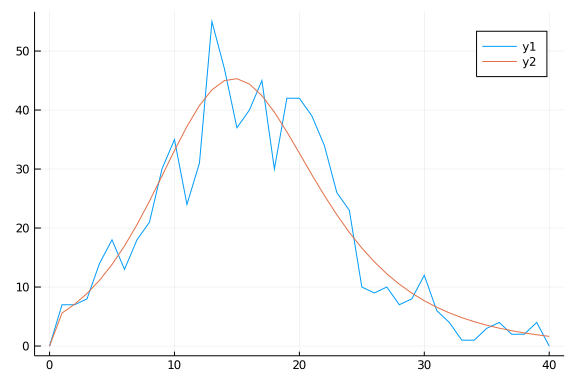
\includegraphics[width=\linewidth]{/home/simon/Projects/sir-julia/pdf/ode/jl_X4tZiv/ode_inference_13_1.pdf}

\subsection{Using Optim.jl directly}

\begin{lstlisting}
(*@\HLJLk{using}@*) (*@\HLJLn{Optim}@*)
\end{lstlisting}


\subsubsection{Single parameter optimization}
This function calculates the sum of squares for a single parameter fit (\ensuremath{\beta}). Note how the original \texttt{ODEProblem} is remade using the \texttt{remake} function.


\begin{lstlisting}
(*@\HLJLk{function}@*) (*@\HLJLnf{ss1}@*)(*@\HLJLp{(}@*)(*@\HLJLn{\ensuremath{\beta}}@*)(*@\HLJLp{)}@*)
    (*@\HLJLn{prob}@*) (*@\HLJLoB{=}@*) (*@\HLJLnf{remake}@*)(*@\HLJLp{(}@*)(*@\HLJLn{prob{\_}ode}@*)(*@\HLJLp{,}@*)(*@\HLJLn{u0}@*)(*@\HLJLoB{=}@*)(*@\HLJLp{[}@*)(*@\HLJLnfB{990.0}@*)(*@\HLJLp{,}@*)(*@\HLJLnfB{10.0}@*)(*@\HLJLp{,}@*)(*@\HLJLnfB{0.0}@*)(*@\HLJLp{,}@*)(*@\HLJLnfB{0.0}@*)(*@\HLJLp{],}@*)(*@\HLJLn{p}@*)(*@\HLJLoB{=}@*)(*@\HLJLp{[}@*)(*@\HLJLn{\ensuremath{\beta}}@*)(*@\HLJLp{,}@*)(*@\HLJLnfB{10.0}@*)(*@\HLJLp{,}@*)(*@\HLJLnfB{0.25}@*)(*@\HLJLp{])}@*)
    (*@\HLJLn{sol}@*) (*@\HLJLoB{=}@*) (*@\HLJLnf{solve}@*)(*@\HLJLp{(}@*)(*@\HLJLn{prob}@*)(*@\HLJLp{,}@*)(*@\HLJLnf{Tsit5}@*)(*@\HLJLp{(),}@*)(*@\HLJLn{callback}@*)(*@\HLJLoB{=}@*)(*@\HLJLn{cb{\_}zero}@*)(*@\HLJLp{,}@*)(*@\HLJLn{saveat}@*)(*@\HLJLoB{=}@*)(*@\HLJLn{obstimes}@*)(*@\HLJLp{)}@*)
    (*@\HLJLn{sol{\_}data}@*) (*@\HLJLoB{=}@*) (*@\HLJLnf{sol}@*)(*@\HLJLp{(}@*)(*@\HLJLn{obstimes}@*)(*@\HLJLp{)[}@*)(*@\HLJLni{4}@*)(*@\HLJLp{,}@*)(*@\HLJLoB{:}@*)(*@\HLJLp{]}@*)
    (*@\HLJLk{return}@*)(*@\HLJLp{(}@*)(*@\HLJLnf{sum}@*)(*@\HLJLp{((}@*)(*@\HLJLn{sol{\_}data}@*) (*@\HLJLoB{-}@*) (*@\HLJLn{data}@*)(*@\HLJLp{)}@*) (*@\HLJLoB{.{\textasciicircum}}@*)(*@\HLJLni{2}@*)(*@\HLJLp{))}@*)
(*@\HLJLk{end}@*)
\end{lstlisting}

\begin{lstlisting}
ss1 (generic function with 1 method)
\end{lstlisting}


Optimisation routines typically \emph{minimise} functions, so for maximum likelihood estimates, we have to define the \emph{negative} log-likelihood - here, for a single parameter, \ensuremath{\beta}.


\begin{lstlisting}
(*@\HLJLk{function}@*) (*@\HLJLnf{nll1}@*)(*@\HLJLp{(}@*)(*@\HLJLn{\ensuremath{\beta}}@*)(*@\HLJLp{)}@*)
    (*@\HLJLn{prob}@*) (*@\HLJLoB{=}@*) (*@\HLJLnf{remake}@*)(*@\HLJLp{(}@*)(*@\HLJLn{prob{\_}ode}@*)(*@\HLJLp{,}@*)(*@\HLJLn{u0}@*)(*@\HLJLoB{=}@*)(*@\HLJLp{[}@*)(*@\HLJLnfB{990.0}@*)(*@\HLJLp{,}@*)(*@\HLJLnfB{10.0}@*)(*@\HLJLp{,}@*)(*@\HLJLnfB{0.0}@*)(*@\HLJLp{,}@*)(*@\HLJLnfB{0.0}@*)(*@\HLJLp{],}@*)(*@\HLJLn{p}@*)(*@\HLJLoB{=}@*)(*@\HLJLp{[}@*)(*@\HLJLn{\ensuremath{\beta}}@*)(*@\HLJLp{,}@*)(*@\HLJLnfB{10.0}@*)(*@\HLJLp{,}@*)(*@\HLJLnfB{0.25}@*)(*@\HLJLp{])}@*)
    (*@\HLJLn{sol}@*) (*@\HLJLoB{=}@*) (*@\HLJLnf{solve}@*)(*@\HLJLp{(}@*)(*@\HLJLn{prob}@*)(*@\HLJLp{,}@*)(*@\HLJLnf{Tsit5}@*)(*@\HLJLp{(),}@*)(*@\HLJLn{callback}@*)(*@\HLJLoB{=}@*)(*@\HLJLn{cb{\_}zero}@*)(*@\HLJLp{,}@*)(*@\HLJLn{saveat}@*)(*@\HLJLoB{=}@*)(*@\HLJLn{obstimes}@*)(*@\HLJLp{)}@*)
    (*@\HLJLn{sol{\_}data}@*) (*@\HLJLoB{=}@*) (*@\HLJLnf{sol}@*)(*@\HLJLp{(}@*)(*@\HLJLn{obstimes}@*)(*@\HLJLp{)[}@*)(*@\HLJLni{4}@*)(*@\HLJLp{,}@*)(*@\HLJLoB{:}@*)(*@\HLJLp{]}@*)
    (*@\HLJLoB{-}@*)(*@\HLJLnf{sum}@*)(*@\HLJLp{(}@*)(*@\HLJLn{logpdf}@*)(*@\HLJLoB{.}@*)(*@\HLJLp{(}@*)(*@\HLJLn{Poisson}@*)(*@\HLJLoB{.}@*)(*@\HLJLp{(}@*)(*@\HLJLn{sol{\_}data}@*)(*@\HLJLp{),}@*)(*@\HLJLn{data}@*)(*@\HLJLp{))}@*)
(*@\HLJLk{end}@*)
\end{lstlisting}

\begin{lstlisting}
nll1 (generic function with 1 method)
\end{lstlisting}


In this model, \ensuremath{\beta} is positive and (through the meaning of the parameter) bounded between 0 and 1. For point estimates, we could use constrained optimisation, or transform \ensuremath{\beta} to an unconstrained scale. Here is the first approach, defining the bounds and initial values for optimization.


\begin{lstlisting}
(*@\HLJLn{lower1}@*) (*@\HLJLoB{=}@*) (*@\HLJLnfB{0.0}@*)
(*@\HLJLn{upper1}@*) (*@\HLJLoB{=}@*) (*@\HLJLnfB{1.0}@*)
(*@\HLJLn{initial{\_}x1}@*) (*@\HLJLoB{=}@*) (*@\HLJLnfB{0.1}@*)
\end{lstlisting}

\begin{lstlisting}
0.1
\end{lstlisting}


Model fit using sum of squares. The output isn't suppressed, as the output of the outcome of the optimisation, such as whether it has converged, is important.


\begin{lstlisting}
(*@\HLJLn{opt1{\_}ss}@*) (*@\HLJLoB{=}@*) (*@\HLJLn{Optim}@*)(*@\HLJLoB{.}@*)(*@\HLJLnf{optimize}@*)(*@\HLJLp{(}@*)(*@\HLJLn{ss1}@*)(*@\HLJLp{,}@*)(*@\HLJLn{lower1}@*)(*@\HLJLp{,}@*)(*@\HLJLn{upper1}@*)(*@\HLJLp{)}@*)
\end{lstlisting}

\begin{lstlisting}
Results of Optimization Algorithm
 * Algorithm: Brent(*@{{\textquotesingle}}@*)s Method
 * Search Interval: [0.000000, 1.000000]
 * Minimizer: 4.915615e-02
 * Minimum: 1.067131e+03
 * Iterations: 13
 * Convergence: max(|x - x(*@{{\_}}@*)upper|, |x - x(*@{{\_}}@*)lower|) <= 2*(1.5e-08*|x|+2.2e-16
): true
 * Objective Function Calls: 14
\end{lstlisting}


Model fit using (negative) log likelihood.


\begin{lstlisting}
(*@\HLJLn{opt1{\_}nll}@*) (*@\HLJLoB{=}@*) (*@\HLJLn{Optim}@*)(*@\HLJLoB{.}@*)(*@\HLJLnf{optimize}@*)(*@\HLJLp{(}@*)(*@\HLJLn{nll1}@*)(*@\HLJLp{,}@*)(*@\HLJLn{lower1}@*)(*@\HLJLp{,}@*)(*@\HLJLn{upper1}@*)(*@\HLJLp{)}@*)
\end{lstlisting}

\begin{lstlisting}
Results of Optimization Algorithm
 * Algorithm: Brent(*@{{\textquotesingle}}@*)s Method
 * Search Interval: [0.000000, 1.000000]
 * Minimizer: 4.976235e-02
 * Minimum: 1.123280e+02
 * Iterations: 19
 * Convergence: max(|x - x(*@{{\_}}@*)upper|, |x - x(*@{{\_}}@*)lower|) <= 2*(1.5e-08*|x|+2.2e-16
): true
 * Objective Function Calls: 20
\end{lstlisting}


\subsubsection{Multiparameter optimization}
Multiple parameters are handled in the cost function using an array argument. Firstly, sum of squares.


\begin{lstlisting}
(*@\HLJLk{function}@*) (*@\HLJLnf{ss2}@*)(*@\HLJLp{(}@*)(*@\HLJLn{x}@*)(*@\HLJLp{)}@*)
    (*@\HLJLp{(}@*)(*@\HLJLn{i0}@*)(*@\HLJLp{,}@*)(*@\HLJLn{\ensuremath{\beta}}@*)(*@\HLJLp{)}@*) (*@\HLJLoB{=}@*) (*@\HLJLn{x}@*)
    (*@\HLJLn{I}@*) (*@\HLJLoB{=}@*) (*@\HLJLn{i0}@*)(*@\HLJLoB{*}@*)(*@\HLJLnfB{1000.0}@*)
    (*@\HLJLn{prob}@*) (*@\HLJLoB{=}@*) (*@\HLJLnf{remake}@*)(*@\HLJLp{(}@*)(*@\HLJLn{prob{\_}ode}@*)(*@\HLJLp{,}@*)(*@\HLJLn{u0}@*)(*@\HLJLoB{=}@*)(*@\HLJLp{[}@*)(*@\HLJLni{1000}@*)(*@\HLJLoB{-}@*)(*@\HLJLn{I}@*)(*@\HLJLp{,}@*)(*@\HLJLn{I}@*)(*@\HLJLp{,}@*)(*@\HLJLnfB{0.0}@*)(*@\HLJLp{,}@*)(*@\HLJLnfB{0.0}@*)(*@\HLJLp{],}@*)(*@\HLJLn{p}@*)(*@\HLJLoB{=}@*)(*@\HLJLp{[}@*)(*@\HLJLn{\ensuremath{\beta}}@*)(*@\HLJLp{,}@*)(*@\HLJLnfB{10.0}@*)(*@\HLJLp{,}@*)(*@\HLJLnfB{0.25}@*)(*@\HLJLp{])}@*)
    (*@\HLJLn{sol}@*) (*@\HLJLoB{=}@*) (*@\HLJLnf{solve}@*)(*@\HLJLp{(}@*)(*@\HLJLn{prob}@*)(*@\HLJLp{,}@*)(*@\HLJLnf{Tsit5}@*)(*@\HLJLp{(),}@*)(*@\HLJLn{callback}@*)(*@\HLJLoB{=}@*)(*@\HLJLn{cb{\_}zero}@*)(*@\HLJLp{,}@*)(*@\HLJLn{saveat}@*)(*@\HLJLoB{=}@*)(*@\HLJLn{obstimes}@*)(*@\HLJLp{)}@*)
    (*@\HLJLn{sol{\_}data}@*) (*@\HLJLoB{=}@*) (*@\HLJLnf{sol}@*)(*@\HLJLp{(}@*)(*@\HLJLn{obstimes}@*)(*@\HLJLp{)[}@*)(*@\HLJLni{4}@*)(*@\HLJLp{,}@*)(*@\HLJLoB{:}@*)(*@\HLJLp{]}@*)
    (*@\HLJLk{return}@*)(*@\HLJLp{(}@*)(*@\HLJLnf{sum}@*)(*@\HLJLp{((}@*)(*@\HLJLn{sol{\_}data}@*) (*@\HLJLoB{-}@*) (*@\HLJLn{data}@*)(*@\HLJLp{)}@*) (*@\HLJLoB{.{\textasciicircum}}@*)(*@\HLJLni{2}@*)(*@\HLJLp{))}@*)
(*@\HLJLk{end}@*)
\end{lstlisting}

\begin{lstlisting}
ss2 (generic function with 1 method)
\end{lstlisting}


Secondly, negative log-likelihood.


\begin{lstlisting}
(*@\HLJLk{function}@*) (*@\HLJLnf{nll2}@*)(*@\HLJLp{(}@*)(*@\HLJLn{x}@*)(*@\HLJLp{)}@*)
    (*@\HLJLp{(}@*)(*@\HLJLn{i0}@*)(*@\HLJLp{,}@*)(*@\HLJLn{\ensuremath{\beta}}@*)(*@\HLJLp{)}@*) (*@\HLJLoB{=}@*) (*@\HLJLn{x}@*)
    (*@\HLJLn{I}@*) (*@\HLJLoB{=}@*) (*@\HLJLn{i0}@*)(*@\HLJLoB{*}@*)(*@\HLJLnfB{1000.0}@*)
    (*@\HLJLn{prob}@*) (*@\HLJLoB{=}@*) (*@\HLJLnf{remake}@*)(*@\HLJLp{(}@*)(*@\HLJLn{prob{\_}ode}@*)(*@\HLJLp{,}@*)(*@\HLJLn{u0}@*)(*@\HLJLoB{=}@*)(*@\HLJLp{[}@*)(*@\HLJLni{1000}@*)(*@\HLJLoB{-}@*)(*@\HLJLn{I}@*)(*@\HLJLp{,}@*)(*@\HLJLn{I}@*)(*@\HLJLp{,}@*)(*@\HLJLnfB{0.0}@*)(*@\HLJLp{,}@*)(*@\HLJLnfB{0.0}@*)(*@\HLJLp{],}@*)(*@\HLJLn{p}@*)(*@\HLJLoB{=}@*)(*@\HLJLp{[}@*)(*@\HLJLn{\ensuremath{\beta}}@*)(*@\HLJLp{,}@*)(*@\HLJLnfB{10.0}@*)(*@\HLJLp{,}@*)(*@\HLJLnfB{0.25}@*)(*@\HLJLp{])}@*)
    (*@\HLJLn{sol}@*) (*@\HLJLoB{=}@*) (*@\HLJLnf{solve}@*)(*@\HLJLp{(}@*)(*@\HLJLn{prob}@*)(*@\HLJLp{,}@*)(*@\HLJLnf{Tsit5}@*)(*@\HLJLp{(),}@*)(*@\HLJLn{callback}@*)(*@\HLJLoB{=}@*)(*@\HLJLn{cb{\_}zero}@*)(*@\HLJLp{,}@*)(*@\HLJLn{saveat}@*)(*@\HLJLoB{=}@*)(*@\HLJLn{obstimes}@*)(*@\HLJLp{)}@*)
    (*@\HLJLn{sol{\_}data}@*) (*@\HLJLoB{=}@*) (*@\HLJLnf{sol}@*)(*@\HLJLp{(}@*)(*@\HLJLn{obstimes}@*)(*@\HLJLp{)[}@*)(*@\HLJLni{4}@*)(*@\HLJLp{,}@*)(*@\HLJLoB{:}@*)(*@\HLJLp{]}@*)
    (*@\HLJLoB{-}@*)(*@\HLJLnf{sum}@*)(*@\HLJLp{(}@*)(*@\HLJLn{logpdf}@*)(*@\HLJLoB{.}@*)(*@\HLJLp{(}@*)(*@\HLJLn{Poisson}@*)(*@\HLJLoB{.}@*)(*@\HLJLp{(}@*)(*@\HLJLn{sol{\_}data}@*)(*@\HLJLp{),}@*)(*@\HLJLn{data}@*)(*@\HLJLp{))}@*)
(*@\HLJLk{end}@*)
\end{lstlisting}

\begin{lstlisting}
nll2 (generic function with 1 method)
\end{lstlisting}


Two-parameter lower and upper bounds and initial conditions.


\begin{lstlisting}
(*@\HLJLn{lower2}@*) (*@\HLJLoB{=}@*) (*@\HLJLp{[}@*)(*@\HLJLnfB{0.0}@*)(*@\HLJLp{,}@*)(*@\HLJLnfB{0.0}@*)(*@\HLJLp{]}@*)
(*@\HLJLn{upper2}@*) (*@\HLJLoB{=}@*) (*@\HLJLp{[}@*)(*@\HLJLnfB{1.0}@*)(*@\HLJLp{,}@*)(*@\HLJLnfB{1.0}@*)(*@\HLJLp{]}@*)
(*@\HLJLn{initial{\_}x2}@*) (*@\HLJLoB{=}@*) (*@\HLJLp{[}@*)(*@\HLJLnfB{0.01}@*)(*@\HLJLp{,}@*)(*@\HLJLnfB{0.1}@*)(*@\HLJLp{]}@*)
\end{lstlisting}

\begin{lstlisting}
2-element Array(*@{{\{}}@*)Float64,1(*@{{\}}}@*):
 0.01
 0.1
\end{lstlisting}


\begin{lstlisting}
(*@\HLJLn{opt2{\_}ss}@*) (*@\HLJLoB{=}@*) (*@\HLJLn{Optim}@*)(*@\HLJLoB{.}@*)(*@\HLJLnf{optimize}@*)(*@\HLJLp{(}@*)(*@\HLJLn{ss2}@*)(*@\HLJLp{,}@*)(*@\HLJLn{lower2}@*)(*@\HLJLp{,}@*)(*@\HLJLn{upper2}@*)(*@\HLJLp{,}@*)(*@\HLJLn{initial{\_}x2}@*)(*@\HLJLp{)}@*)
\end{lstlisting}

\begin{lstlisting}
* Status: success

 * Candidate solution
    Minimizer: [9.03e-03, 4.97e-02]
    Minimum:   1.050409e+03

 * Found with
    Algorithm:     Fminbox with L-BFGS
    Initial Point: [1.00e-02, 1.00e-01]

 * Convergence measures
    |x - x(*@{{\textquotesingle}}@*)|               = 0.00e+00 (*@\ensuremath{\le}@*) 0.0e+00
    |x - x(*@{{\textquotesingle}}@*)|/|x(*@{{\textquotesingle}}@*)|          = 0.00e+00 (*@\ensuremath{\le}@*) 0.0e+00
    |f(x) - f(x(*@{{\textquotesingle}}@*))|         = 0.00e+00 (*@\ensuremath{\le}@*) 0.0e+00
    |f(x) - f(x(*@{{\textquotesingle}}@*))|/|f(x(*@{{\textquotesingle}}@*))| = 0.00e+00 (*@\ensuremath{\le}@*) 0.0e+00
    |g(x)|                 = 1.22e-03 (*@\ensuremath{\nleq}@*) 1.0e-08

 * Work counters
    Seconds run:   0  (vs limit Inf)
    Iterations:    4
    f(x) calls:    241
    (*@\ensuremath{\del}@*)f(x) calls:   241
\end{lstlisting}


\begin{lstlisting}
(*@\HLJLn{opt2{\_}nll}@*) (*@\HLJLoB{=}@*) (*@\HLJLn{Optim}@*)(*@\HLJLoB{.}@*)(*@\HLJLnf{optimize}@*)(*@\HLJLp{(}@*)(*@\HLJLn{nll2}@*)(*@\HLJLp{,}@*)(*@\HLJLn{lower2}@*)(*@\HLJLp{,}@*)(*@\HLJLn{upper2}@*)(*@\HLJLp{,}@*)(*@\HLJLn{initial{\_}x2}@*)(*@\HLJLp{)}@*)
\end{lstlisting}

\begin{lstlisting}
* Status: success

 * Candidate solution
    Minimizer: [9.46e-03, 5.01e-02]
    Minimum:   1.122337e+02

 * Found with
    Algorithm:     Fminbox with L-BFGS
    Initial Point: [1.00e-02, 1.00e-01]

 * Convergence measures
    |x - x(*@{{\textquotesingle}}@*)|               = 0.00e+00 (*@\ensuremath{\le}@*) 0.0e+00
    |x - x(*@{{\textquotesingle}}@*)|/|x(*@{{\textquotesingle}}@*)|          = 0.00e+00 (*@\ensuremath{\le}@*) 0.0e+00
    |f(x) - f(x(*@{{\textquotesingle}}@*))|         = 0.00e+00 (*@\ensuremath{\le}@*) 0.0e+00
    |f(x) - f(x(*@{{\textquotesingle}}@*))|/|f(x(*@{{\textquotesingle}}@*))| = 0.00e+00 (*@\ensuremath{\le}@*) 0.0e+00
    |g(x)|                 = 4.48e-05 (*@\ensuremath{\nleq}@*) 1.0e-08

 * Work counters
    Seconds run:   0  (vs limit Inf)
    Iterations:    4
    f(x) calls:    268
    (*@\ensuremath{\del}@*)f(x) calls:   268
\end{lstlisting}


\subsection{Using DiffEqParamEstim}
The advantage of using a framework such as DiffEqParamEstim is that a number of different frameworks can be employed easily. Firstly, the loss function is defined.


\begin{lstlisting}
(*@\HLJLk{function}@*) (*@\HLJLnf{loss{\_}function}@*)(*@\HLJLp{(}@*)(*@\HLJLn{sol}@*)(*@\HLJLp{)}@*)
    (*@\HLJLn{sol{\_}data}@*) (*@\HLJLoB{=}@*) (*@\HLJLnf{DataFrame}@*)(*@\HLJLp{(}@*)(*@\HLJLnf{sol}@*)(*@\HLJLp{(}@*)(*@\HLJLn{obstimes}@*)(*@\HLJLp{)}@*)(*@\HLJLoB{{\textquotesingle}}@*)(*@\HLJLp{)[}@*)(*@\HLJLoB{!}@*)(*@\HLJLp{,}@*)(*@\HLJLoB{:}@*)(*@\HLJLn{x4}@*)(*@\HLJLp{]}@*)
    (*@\HLJLoB{-}@*)(*@\HLJLnf{sum}@*)(*@\HLJLp{(}@*)(*@\HLJLn{logpdf}@*)(*@\HLJLoB{.}@*)(*@\HLJLp{(}@*)(*@\HLJLn{Poisson}@*)(*@\HLJLoB{.}@*)(*@\HLJLp{(}@*)(*@\HLJLn{sol{\_}data}@*)(*@\HLJLp{),}@*)(*@\HLJLn{data}@*)(*@\HLJLp{))}@*)
(*@\HLJLk{end}@*)
\end{lstlisting}

\begin{lstlisting}
loss(*@{{\_}}@*)function (generic function with 1 method)
\end{lstlisting}


Secondly, a function that generates the \texttt{Problem} to be solved.


\begin{lstlisting}
(*@\HLJLn{prob{\_}generator}@*) (*@\HLJLoB{=}@*) (*@\HLJLp{(}@*)(*@\HLJLn{prob}@*)(*@\HLJLp{,}@*)(*@\HLJLn{q}@*)(*@\HLJLp{)}@*) (*@\HLJLoB{->}@*) (*@\HLJLnf{remake}@*)(*@\HLJLp{(}@*)(*@\HLJLn{prob}@*)(*@\HLJLp{,}@*)
    (*@\HLJLn{u0}@*)(*@\HLJLoB{=}@*)(*@\HLJLp{[}@*)(*@\HLJLni{1000}@*)(*@\HLJLoB{-}@*)(*@\HLJLp{(}@*)(*@\HLJLn{q}@*)(*@\HLJLp{[}@*)(*@\HLJLni{1}@*)(*@\HLJLp{]}@*)(*@\HLJLoB{*}@*)(*@\HLJLni{1000}@*)(*@\HLJLp{),}@*)(*@\HLJLn{q}@*)(*@\HLJLp{[}@*)(*@\HLJLni{1}@*)(*@\HLJLp{]}@*)(*@\HLJLoB{*}@*)(*@\HLJLni{1000}@*)(*@\HLJLp{,}@*)(*@\HLJLnfB{0.0}@*)(*@\HLJLp{,}@*)(*@\HLJLnfB{0.0}@*)(*@\HLJLp{],}@*)
    (*@\HLJLn{p}@*)(*@\HLJLoB{=}@*)(*@\HLJLp{[}@*)(*@\HLJLn{q}@*)(*@\HLJLp{[}@*)(*@\HLJLni{2}@*)(*@\HLJLp{],}@*)(*@\HLJLnfB{10.0}@*)(*@\HLJLp{,}@*)(*@\HLJLnfB{0.25}@*)(*@\HLJLp{])}@*)
\end{lstlisting}

\begin{lstlisting}
(*@{{\#}}@*)3 (generic function with 1 method)
\end{lstlisting}


The loss function and the problem generator then get combined to build the objective function.


\begin{lstlisting}
(*@\HLJLn{cost{\_}function}@*) (*@\HLJLoB{=}@*) (*@\HLJLnf{build{\_}loss{\_}objective}@*)(*@\HLJLp{(}@*)(*@\HLJLn{prob{\_}ode}@*)(*@\HLJLp{,}@*)
    (*@\HLJLnf{Tsit5}@*)(*@\HLJLp{(),}@*)
    (*@\HLJLn{loss{\_}function}@*)(*@\HLJLp{,}@*)
    (*@\HLJLn{prob{\_}generator}@*) (*@\HLJLoB{=}@*) (*@\HLJLn{prob{\_}generator}@*)(*@\HLJLp{,}@*)
    (*@\HLJLn{maxiters}@*)(*@\HLJLoB{=}@*)(*@\HLJLni{10000}@*)(*@\HLJLp{,}@*)
    (*@\HLJLn{verbose}@*)(*@\HLJLoB{=}@*)(*@\HLJLkc{false}@*)(*@\HLJLp{,}@*)
    (*@\HLJLn{callback}@*)(*@\HLJLoB{=}@*)(*@\HLJLn{cb{\_}zero}@*)(*@\HLJLp{)}@*)
\end{lstlisting}

\begin{lstlisting}
(::DiffEqObjective(*@{{\{}}@*)DiffEqParamEstim.var(*@{"{}}@*)(*@{{\#}}@*)43(*@{{\#}}@*)48(*@{"{}}@*)(*@{{\{}}@*)Nothing,Bool,Int64,Main.(*@{{\#}}@*)(*@{{\#}}@*)W
eaveSandBox(*@{{\#}}@*)993.var(*@{"{}}@*)(*@{{\#}}@*)3(*@{{\#}}@*)4(*@{"{}}@*),Base.Iterators.Pairs(*@{{\{}}@*)Symbol,Any,Tuple(*@{{\{}}@*)Symbol,Symb
ol,Symbol(*@{{\}}}@*),NamedTuple(*@{{\{}}@*)(:maxiters, :verbose, :callback),Tuple(*@{{\{}}@*)Int64,Bool,Dis
creteCallback(*@{{\{}}@*)DiffEqCallbacks.var(*@{"{}}@*)(*@{{\#}}@*)53(*@{{\#}}@*)56(*@{"{}}@*)(*@{{\{}}@*)StepRangeLen(*@{{\{}}@*)Float64,Base.TwicePr
ecision(*@{{\{}}@*)Float64(*@{{\}}}@*),Base.TwicePrecision(*@{{\{}}@*)Float64(*@{{\}}}@*)(*@{{\}}}@*)(*@{{\}}}@*),DiffEqCallbacks.var(*@{"{}}@*)(*@{{\#}}@*)54(*@{{\#}}@*)57(*@{"{}}@*)
(*@{{\{}}@*)typeof(Main.(*@{{\#}}@*)(*@{{\#}}@*)WeaveSandBox(*@{{\#}}@*)993.affect!)(*@{{\}}}@*),DiffEqCallbacks.var(*@{"{}}@*)(*@{{\#}}@*)55(*@{{\#}}@*)58(*@{"{}}@*)(*@{{\{}}@*)typeo
f(DiffEqBase.INITIALIZE(*@{{\_}}@*)DEFAULT),Bool,StepRangeLen(*@{{\{}}@*)Float64,Base.TwicePrecis
ion(*@{{\{}}@*)Float64(*@{{\}}}@*),Base.TwicePrecision(*@{{\{}}@*)Float64(*@{{\}}}@*)(*@{{\}}}@*),typeof(Main.(*@{{\#}}@*)(*@{{\#}}@*)WeaveSandBox(*@{{\#}}@*)993.a
ffect!)(*@{{\}}}@*)(*@{{\}}}@*)(*@{{\}}}@*)(*@{{\}}}@*)(*@{{\}}}@*),ODEProblem(*@{{\{}}@*)Array(*@{{\{}}@*)Float64,1(*@{{\}}}@*),Tuple(*@{{\{}}@*)Float64,Float64(*@{{\}}}@*),true,Array(*@{{\{}}@*)
Float64,1(*@{{\}}}@*),ODEFunction(*@{{\{}}@*)true,typeof(Main.(*@{{\#}}@*)(*@{{\#}}@*)WeaveSandBox(*@{{\#}}@*)993.sir(*@{{\_}}@*)ode!),Linear
Algebra.UniformScaling(*@{{\{}}@*)Bool(*@{{\}}}@*),Nothing,Nothing,Nothing,Nothing,Nothing,Nothin
g,Nothing,Nothing,Nothing,Nothing,Nothing,Nothing(*@{{\}}}@*),Base.Iterators.Pairs(*@{{\{}}@*)Uni
on(*@{{\{}}@*)(*@{{\}}}@*),Union(*@{{\{}}@*)(*@{{\}}}@*),Tuple(*@{{\{}}@*)(*@{{\}}}@*),NamedTuple(*@{{\{}}@*)(),Tuple(*@{{\{}}@*)(*@{{\}}}@*)(*@{{\}}}@*)(*@{{\}}}@*),DiffEqBase.StandardODEProblem(*@{{\}}}@*)
,Tsit5,typeof(Main.(*@{{\#}}@*)(*@{{\#}}@*)WeaveSandBox(*@{{\#}}@*)993.loss(*@{{\_}}@*)function),Nothing(*@{{\}}}@*),DiffEqParamEs
tim.var(*@{"{}}@*)(*@{{\#}}@*)47(*@{{\#}}@*)53(*@{"{}}@*)(*@{{\{}}@*)DiffEqParamEstim.var(*@{"{}}@*)(*@{{\#}}@*)43(*@{{\#}}@*)48(*@{"{}}@*)(*@{{\{}}@*)Nothing,Bool,Int64,Main.(*@{{\#}}@*)(*@{{\#}}@*)Weav
eSandBox(*@{{\#}}@*)993.var(*@{"{}}@*)(*@{{\#}}@*)3(*@{{\#}}@*)4(*@{"{}}@*),Base.Iterators.Pairs(*@{{\{}}@*)Symbol,Any,Tuple(*@{{\{}}@*)Symbol,Symbol,
Symbol(*@{{\}}}@*),NamedTuple(*@{{\{}}@*)(:maxiters, :verbose, :callback),Tuple(*@{{\{}}@*)Int64,Bool,Discre
teCallback(*@{{\{}}@*)DiffEqCallbacks.var(*@{"{}}@*)(*@{{\#}}@*)53(*@{{\#}}@*)56(*@{"{}}@*)(*@{{\{}}@*)StepRangeLen(*@{{\{}}@*)Float64,Base.TwicePreci
sion(*@{{\{}}@*)Float64(*@{{\}}}@*),Base.TwicePrecision(*@{{\{}}@*)Float64(*@{{\}}}@*)(*@{{\}}}@*)(*@{{\}}}@*),DiffEqCallbacks.var(*@{"{}}@*)(*@{{\#}}@*)54(*@{{\#}}@*)57(*@{"{}}@*)(*@{{\{}}@*)ty
peof(Main.(*@{{\#}}@*)(*@{{\#}}@*)WeaveSandBox(*@{{\#}}@*)993.affect!)(*@{{\}}}@*),DiffEqCallbacks.var(*@{"{}}@*)(*@{{\#}}@*)55(*@{{\#}}@*)58(*@{"{}}@*)(*@{{\{}}@*)typeof(D
iffEqBase.INITIALIZE(*@{{\_}}@*)DEFAULT),Bool,StepRangeLen(*@{{\{}}@*)Float64,Base.TwicePrecision
(*@{{\{}}@*)Float64(*@{{\}}}@*),Base.TwicePrecision(*@{{\{}}@*)Float64(*@{{\}}}@*)(*@{{\}}}@*),typeof(Main.(*@{{\#}}@*)(*@{{\#}}@*)WeaveSandBox(*@{{\#}}@*)993.affe
ct!)(*@{{\}}}@*)(*@{{\}}}@*)(*@{{\}}}@*)(*@{{\}}}@*)(*@{{\}}}@*),ODEProblem(*@{{\{}}@*)Array(*@{{\{}}@*)Float64,1(*@{{\}}}@*),Tuple(*@{{\{}}@*)Float64,Float64(*@{{\}}}@*),true,Array(*@{{\{}}@*)Flo
at64,1(*@{{\}}}@*),ODEFunction(*@{{\{}}@*)true,typeof(Main.(*@{{\#}}@*)(*@{{\#}}@*)WeaveSandBox(*@{{\#}}@*)993.sir(*@{{\_}}@*)ode!),LinearAlg
ebra.UniformScaling(*@{{\{}}@*)Bool(*@{{\}}}@*),Nothing,Nothing,Nothing,Nothing,Nothing,Nothing,N
othing,Nothing,Nothing,Nothing,Nothing,Nothing(*@{{\}}}@*),Base.Iterators.Pairs(*@{{\{}}@*)Union(*@{{\{}}@*)
(*@{{\}}}@*),Union(*@{{\{}}@*)(*@{{\}}}@*),Tuple(*@{{\{}}@*)(*@{{\}}}@*),NamedTuple(*@{{\{}}@*)(),Tuple(*@{{\{}}@*)(*@{{\}}}@*)(*@{{\}}}@*)(*@{{\}}}@*),DiffEqBase.StandardODEProblem(*@{{\}}}@*),Ts
it5,typeof(Main.(*@{{\#}}@*)(*@{{\#}}@*)WeaveSandBox(*@{{\#}}@*)993.loss(*@{{\_}}@*)function),Nothing(*@{{\}}}@*)(*@{{\}}}@*)(*@{{\}}}@*)) (generic func
tion with 2 methods)
\end{lstlisting}


\subsubsection{Optim interface}
The resulting cost function can be passed to \texttt{Optim.jl} as before.


\begin{lstlisting}
(*@\HLJLn{opt{\_}pe1}@*) (*@\HLJLoB{=}@*) (*@\HLJLn{Optim}@*)(*@\HLJLoB{.}@*)(*@\HLJLnf{optimize}@*)(*@\HLJLp{(}@*)(*@\HLJLn{cost{\_}function}@*)(*@\HLJLp{,}@*)(*@\HLJLn{lower2}@*)(*@\HLJLp{,}@*)(*@\HLJLn{upper2}@*)(*@\HLJLp{,}@*)(*@\HLJLn{initial{\_}x2}@*)(*@\HLJLp{)}@*)
\end{lstlisting}

\begin{lstlisting}
* Status: success

 * Candidate solution
    Minimizer: [9.46e-03, 5.01e-02]
    Minimum:   1.122337e+02

 * Found with
    Algorithm:     Fminbox with L-BFGS
    Initial Point: [1.00e-02, 1.00e-01]

 * Convergence measures
    |x - x(*@{{\textquotesingle}}@*)|               = 0.00e+00 (*@\ensuremath{\le}@*) 0.0e+00
    |x - x(*@{{\textquotesingle}}@*)|/|x(*@{{\textquotesingle}}@*)|          = 0.00e+00 (*@\ensuremath{\le}@*) 0.0e+00
    |f(x) - f(x(*@{{\textquotesingle}}@*))|         = 0.00e+00 (*@\ensuremath{\le}@*) 0.0e+00
    |f(x) - f(x(*@{{\textquotesingle}}@*))|/|f(x(*@{{\textquotesingle}}@*))| = 0.00e+00 (*@\ensuremath{\le}@*) 0.0e+00
    |g(x)|                 = 4.66e-05 (*@\ensuremath{\nleq}@*) 1.0e-08

 * Work counters
    Seconds run:   2  (vs limit Inf)
    Iterations:    4
    f(x) calls:    245
    (*@\ensuremath{\del}@*)f(x) calls:   245
\end{lstlisting}


\subsubsection{NLopt interface}
The same function can also be passed to \texttt{NLopt.jl}.


\begin{lstlisting}
(*@\HLJLk{using}@*) (*@\HLJLn{NLopt}@*)
(*@\HLJLn{opt}@*) (*@\HLJLoB{=}@*) (*@\HLJLnf{Opt}@*)(*@\HLJLp{(}@*)(*@\HLJLsc{:LD{\_}MMA}@*)(*@\HLJLp{,}@*) (*@\HLJLni{2}@*)(*@\HLJLp{)}@*)
(*@\HLJLn{opt}@*)(*@\HLJLoB{.}@*)(*@\HLJLn{lower{\_}bounds}@*) (*@\HLJLoB{=}@*) (*@\HLJLn{lower2}@*)
(*@\HLJLn{opt}@*)(*@\HLJLoB{.}@*)(*@\HLJLn{upper{\_}bounds}@*) (*@\HLJLoB{=}@*) (*@\HLJLn{upper2}@*)
(*@\HLJLn{opt}@*)(*@\HLJLoB{.}@*)(*@\HLJLn{min{\_}objective}@*) (*@\HLJLoB{=}@*) (*@\HLJLn{cost{\_}function}@*)
(*@\HLJLp{(}@*)(*@\HLJLn{minf}@*)(*@\HLJLp{,}@*)(*@\HLJLn{minx}@*)(*@\HLJLp{,}@*)(*@\HLJLn{ret}@*)(*@\HLJLp{)}@*) (*@\HLJLoB{=}@*) (*@\HLJLn{NLopt}@*)(*@\HLJLoB{.}@*)(*@\HLJLnf{optimize}@*)(*@\HLJLp{(}@*)(*@\HLJLn{opt}@*)(*@\HLJLp{,}@*)(*@\HLJLn{initial{\_}x2}@*)(*@\HLJLp{)}@*)
\end{lstlisting}

\begin{lstlisting}
(1716.3967612401862, [0.01, 0.1], :FORCED(*@{{\_}}@*)STOP)
\end{lstlisting}


\subsubsection{BlackBoxOptim interface}
We can also use \texttt{BlackBoxOptim.jl}.


\begin{lstlisting}
(*@\HLJLk{using}@*) (*@\HLJLn{BlackBoxOptim}@*)
(*@\HLJLn{bound1}@*) (*@\HLJLoB{=}@*) (*@\HLJLnf{Tuple}@*)(*@\HLJLp{{\{}}@*)(*@\HLJLn{Float64}@*)(*@\HLJLp{,}@*) (*@\HLJLn{Float64}@*)(*@\HLJLp{{\}}[(}@*)(*@\HLJLnfB{0.0}@*)(*@\HLJLp{,}@*)(*@\HLJLnfB{1.0}@*)(*@\HLJLp{),(}@*)(*@\HLJLnfB{0.0}@*)(*@\HLJLp{,}@*) (*@\HLJLnfB{1.0}@*)(*@\HLJLp{)]}@*)
(*@\HLJLn{result}@*) (*@\HLJLoB{=}@*) (*@\HLJLnf{bboptimize}@*)(*@\HLJLp{(}@*)(*@\HLJLn{cost{\_}function}@*)(*@\HLJLp{;}@*)(*@\HLJLn{SearchRange}@*) (*@\HLJLoB{=}@*) (*@\HLJLn{bound1}@*)(*@\HLJLp{,}@*) (*@\HLJLn{MaxSteps}@*) (*@\HLJLoB{=}@*) (*@\HLJLnfB{110e3}@*)(*@\HLJLp{)}@*)
\end{lstlisting}

\begin{lstlisting}
Starting optimization with optimizer DiffEvoOpt(*@{{\{}}@*)FitPopulation(*@{{\{}}@*)Float64(*@{{\}}}@*),Radi
usLimitedSelector,BlackBoxOptim.AdaptiveDiffEvoRandBin(*@{{\{}}@*)3(*@{{\}}}@*),RandomBound(*@{{\{}}@*)Conti
nuousRectSearchSpace(*@{{\}}}@*)(*@{{\}}}@*)
0.00 secs, 0 evals, 0 steps
0.51 secs, 1657 evals, 1550 steps, improv/step: 0.334 (last = 0.3342), fitn
ess=112.298121563
1.01 secs, 3055 evals, 2948 steps, improv/step: 0.312 (last = 0.2876), fitn
ess=112.233654108
1.54 secs, 4300 evals, 4193 steps, improv/step: 0.297 (last = 0.2618), fitn
ess=112.233653347
2.04 secs, 6581 evals, 6476 steps, improv/step: 0.266 (last = 0.2081), fitn
ess=112.233653346
2.54 secs, 8971 evals, 8866 steps, improv/step: 0.205 (last = 0.0410), fitn
ess=112.233653346
3.04 secs, 11252 evals, 11149 steps, improv/step: 0.169 (last = 0.0267), fi
tness=112.233653346
3.54 secs, 13503 evals, 13618 steps, improv/step: 0.143 (last = 0.0255), fi
tness=112.233653346

Optimization stopped after 15774 steps and 3.77 seconds
Termination reason: Too many steps (101) without any function evaluations (
probably search has converged)
Steps per second = 4188.28
Function evals per second = 3882.93
Improvements/step = 0.01859
Total function evaluations = 14624


Best candidate found: [0.00946262, 0.0501321]

Fitness: 112.233653346

BlackBoxOptim.OptimizationResults((*@{"{}}@*)adaptive(*@{{\_}}@*)de(*@{{\_}}@*)rand(*@{{\_}}@*)1(*@{{\_}}@*)bin(*@{{\_}}@*)radiuslimited(*@{"{}}@*), (*@{"{}}@*)
Too many steps (101) without any function evaluations (probably search has 
converged)(*@{"{}}@*), 15774, 1.590105798403305e9, 3.766223907470703, DictChain(*@{{\{}}@*)Symbo
l,Any(*@{{\}}}@*)[DictChain(*@{{\{}}@*)Symbol,Any(*@{{\}}}@*)[Dict(*@{{\{}}@*)Symbol,Any(*@{{\}}}@*)(:RngSeed => 446022,:SearchRan
ge => [(0.0, 1.0), (0.0, 1.0)],:MaxSteps => 110000),Dict(*@{{\{}}@*)Symbol,Any(*@{{\}}}@*)()],Dic
t(*@{{\{}}@*)Symbol,Any(*@{{\}}}@*)(:FitnessScheme => ScalarFitnessScheme(*@{{\{}}@*)true(*@{{\}}}@*)(),:NumDimensions 
=> :NotSpecified,:PopulationSize => 50,:MaxTime => 0.0,:SearchRange => (-1.
0, 1.0),:Method => :adaptive(*@{{\_}}@*)de(*@{{\_}}@*)rand(*@{{\_}}@*)1(*@{{\_}}@*)bin(*@{{\_}}@*)radiuslimited,:MaxNumStepsWithou
tFuncEvals => 100,:RngSeed => 1234,:MaxFuncEvals => 0,:SaveTrace => false(*@\ensuremath{\dots}@*))
], 14624, ScalarFitnessScheme(*@{{\{}}@*)true(*@{{\}}}@*)(), BlackBoxOptim.TopListArchiveOutput(*@{{\{}}@*)F
loat64,Array(*@{{\{}}@*)Float64,1(*@{{\}}}@*)(*@{{\}}}@*)(112.23365334613528, [0.009462624392968525, 0.05013
21061410536]), BlackBoxOptim.PopulationOptimizerOutput(*@{{\{}}@*)FitPopulation(*@{{\{}}@*)Float6
4(*@{{\}}}@*)(*@{{\}}}@*)(FitPopulation(*@{{\{}}@*)Float64(*@{{\}}}@*)([0.009462624392968525 0.009462624392968525 (*@\ensuremath{\dots}@*) 0.0
09462624392968525 0.009462624392968525; 0.0501321061410536 0.05013210614105
36 (*@\ensuremath{\dots}@*) 0.0501321061410536 0.0501321061410536], NaN, [112.23365334613528, 112.
23365334613528, 112.23365334613528, 112.23365334613528, 112.23365334613528,
 112.23365334613528, 112.23365334613528, 112.23365334613528, 112.2336533461
3528, 112.23365334613528  (*@\ensuremath{\dots}@*)  112.23365334613528, 112.23365334613528, 112.23
365334613528, 112.23365334613528, 112.23365334613528, 112.23365334613528, 1
12.23365334613528, 112.23365334613528, 112.23365334613528, 112.233653346135
28], 0, BlackBoxOptim.Candidate(*@{{\{}}@*)Float64(*@{{\}}}@*)[BlackBoxOptim.Candidate(*@{{\{}}@*)Float64(*@{{\}}}@*)([
0.009462624392968525, 0.0501321061410536], 42, 112.23365334613528, BlackBox
Optim.AdaptiveDiffEvoRandBin(*@{{\{}}@*)3(*@{{\}}}@*)(BlackBoxOptim.AdaptiveDiffEvoParameters(Bla
ckBoxOptim.BimodalCauchy(Cauchy(*@{{\{}}@*)Float64(*@{{\}}}@*)((*@\ensuremath{\mu}@*)=0.65, (*@\ensuremath{\sigma}@*)=0.1), Cauchy(*@{{\{}}@*)Float64(*@{{\}}}@*)((*@\ensuremath{\mu}@*)=
1.0, (*@\ensuremath{\sigma}@*)=0.1), 0.5, false, true), BlackBoxOptim.BimodalCauchy(Cauchy(*@{{\{}}@*)Float64(*@{{\}}}@*)
((*@\ensuremath{\mu}@*)=0.1, (*@\ensuremath{\sigma}@*)=0.1), Cauchy(*@{{\{}}@*)Float64(*@{{\}}}@*)((*@\ensuremath{\mu}@*)=0.95, (*@\ensuremath{\sigma}@*)=0.1), 0.5, false, true), [0.23862
954336539, 1.0, 1.0, 0.409248966683194, 1.0, 0.46710344093721723, 0.9362174
082339615, 0.6626759608325512, 0.8626712321476566, 1.0  (*@\ensuremath{\dots}@*)  0.96761024724919
39, 1.0, 0.6419764185097911, 1.0, 1.0, 1.0, 0.7993844981504739, 0.372123427
49585825, 1.0, 0.8520895347823638], [0.555411051231026, 0.9003285997401819,
 0.8587265247295177, 1.0, 1.0, 0.1758404013462551, 0.06883248929044317, 0.9
759315985173317, 1.0, 0.040963746882380615  (*@\ensuremath{\dots}@*)  0.9018879007447549, 0.060719
45926632988, 0.8992750545302876, 1.0, 1.0, 0.7844953522916855, 0.3195253133
354813, 1.0, 0.7421939033423076, 0.8365800952018762])), 0), BlackBoxOptim.C
andidate(*@{{\{}}@*)Float64(*@{{\}}}@*)([0.009462624392968525, 0.0501321061410536], 42, 112.23365
334613528, BlackBoxOptim.AdaptiveDiffEvoRandBin(*@{{\{}}@*)3(*@{{\}}}@*)(BlackBoxOptim.AdaptiveDi
ffEvoParameters(BlackBoxOptim.BimodalCauchy(Cauchy(*@{{\{}}@*)Float64(*@{{\}}}@*)((*@\ensuremath{\mu}@*)=0.65, (*@\ensuremath{\sigma}@*)=0.1),
 Cauchy(*@{{\{}}@*)Float64(*@{{\}}}@*)((*@\ensuremath{\mu}@*)=1.0, (*@\ensuremath{\sigma}@*)=0.1), 0.5, false, true), BlackBoxOptim.BimodalCau
chy(Cauchy(*@{{\{}}@*)Float64(*@{{\}}}@*)((*@\ensuremath{\mu}@*)=0.1, (*@\ensuremath{\sigma}@*)=0.1), Cauchy(*@{{\{}}@*)Float64(*@{{\}}}@*)((*@\ensuremath{\mu}@*)=0.95, (*@\ensuremath{\sigma}@*)=0.1), 0.5, fal
se, true), [0.23862954336539, 1.0, 1.0, 0.409248966683194, 1.0, 0.467103440
93721723, 0.9362174082339615, 0.6626759608325512, 0.8626712321476566, 1.0  
(*@\ensuremath{\dots}@*)  0.9676102472491939, 1.0, 0.6419764185097911, 1.0, 1.0, 1.0, 0.7993844981
504739, 0.37212342749585825, 1.0, 0.8520895347823638], [0.555411051231026, 
0.9003285997401819, 0.8587265247295177, 1.0, 1.0, 0.1758404013462551, 0.068
83248929044317, 0.9759315985173317, 1.0, 0.040963746882380615  (*@\ensuremath{\dots}@*)  0.9018879
007447549, 0.06071945926632988, 0.8992750545302876, 1.0, 1.0, 0.78449535229
16855, 0.3195253133354813, 1.0, 0.7421939033423076, 0.8365800952018762])), 
0)])))
\end{lstlisting}



\subsection{Appendix}

\subsubsection{Computer Information}

\begin{verbatim}
Julia Version 1.4.1
Commit 381693d3df* (2020-04-14 17:20 UTC)
Platform Info:
  OS: Linux (x86_64-pc-linux-gnu)
  CPU: Intel(R) Core(TM) i7-1065G7 CPU @ 1.30GHz
  WORD_SIZE: 64
  LIBM: libopenlibm
  LLVM: libLLVM-8.0.1 (ORCJIT, icelake-client)
Environment:
  JULIA_NUM_THREADS = 4

\end{verbatim}

\subsubsection{Package Information}

\begin{verbatim}
Status `~/.julia/environments/v1.4/Project.toml`
[46ada45e-f475-11e8-01d0-f70cc89e6671] Agents 3.1.0
[c52e3926-4ff0-5f6e-af25-54175e0327b1] Atom 0.12.11
[6e4b80f9-dd63-53aa-95a3-0cdb28fa8baf] BenchmarkTools 0.5.0
[a134a8b2-14d6-55f6-9291-3336d3ab0209] BlackBoxOptim 0.5.0
[2445eb08-9709-466a-b3fc-47e12bd697a2] DataDrivenDiffEq 0.2.0
[a93c6f00-e57d-5684-b7b6-d8193f3e46c0] DataFrames 0.21.0
[ebbdde9d-f333-5424-9be2-dbf1e9acfb5e] DiffEqBayes 2.14.0
[459566f4-90b8-5000-8ac3-15dfb0a30def] DiffEqCallbacks 2.13.2
[c894b116-72e5-5b58-be3c-e6d8d4ac2b12] DiffEqJump 6.7.5
[1130ab10-4a5a-5621-a13d-e4788d82bd4c] DiffEqParamEstim 1.14.1
[0c46a032-eb83-5123-abaf-570d42b7fbaa] DifferentialEquations 6.14.0
[31c24e10-a181-5473-b8eb-7969acd0382f] Distributions 0.23.2
[634d3b9d-ee7a-5ddf-bec9-22491ea816e1] DrWatson 1.11.0
[587475ba-b771-5e3f-ad9e-33799f191a9c] Flux 0.8.3
[28b8d3ca-fb5f-59d9-8090-bfdbd6d07a71] GR 0.49.1
[523d8e89-b243-5607-941c-87d699ea6713] Gillespie 0.1.0
[7073ff75-c697-5162-941a-fcdaad2a7d2a] IJulia 1.21.2
[4076af6c-e467-56ae-b986-b466b2749572] JuMP 0.21.2
[e5e0dc1b-0480-54bc-9374-aad01c23163d] Juno 0.8.2
[093fc24a-ae57-5d10-9952-331d41423f4d] LightGraphs 1.3.3
[1914dd2f-81c6-5fcd-8719-6d5c9610ff09] MacroTools 0.5.5
[ee78f7c6-11fb-53f2-987a-cfe4a2b5a57a] Makie 0.9.5
[961ee093-0014-501f-94e3-6117800e7a78] ModelingToolkit 3.6.0
[76087f3c-5699-56af-9a33-bf431cd00edd] NLopt 0.6.0
[429524aa-4258-5aef-a3af-852621145aeb] Optim 0.21.0
[1dea7af3-3e70-54e6-95c3-0bf5283fa5ed] OrdinaryDiffEq 5.38.1
[91a5bcdd-55d7-5caf-9e0b-520d859cae80] Plots 1.3.1
[428bdadb-6287-5aa5-874b-9969638295fd] SimJulia 0.8.0
[05bca326-078c-5bf0-a5bf-ce7c7982d7fd] SimpleDiffEq 1.1.0
[f3b207a7-027a-5e70-b257-86293d7955fd] StatsPlots 0.14.6
[789caeaf-c7a9-5a7d-9973-96adeb23e2a0] StochasticDiffEq 6.23.0
[fce5fe82-541a-59a6-adf8-730c64b5f9a0] Turing 0.12.0
[44d3d7a6-8a23-5bf8-98c5-b353f8df5ec9] Weave 0.10.0
\end{verbatim}



\end{document}
